\documentclass{article}
\usepackage[margin=1in]{geometry}
\usepackage{amsmath,amsthm,amssymb}
\usepackage{bbm,enumerate,mathtools}
\usepackage{tikz,pgfplots}
\usepackage{chessboard}
\usepackage[hidelinks]{hyperref}
\usepackage{multicol} % Problem 35
\usepackage{xstring} % Difficulty command
\usetikzlibrary{shapes.geometric}

\newenvironment{question}{\begin{trivlist}\item[\textbf{Question.}]}{\end{trivlist}}
\newenvironment{note}{\begin{trivlist}\item[\textbf{Note.}]}{\end{trivlist}}
\newenvironment{references}{\begin{trivlist}\item[\textbf{References.}]}{\end{trivlist}}
\newenvironment{related}{\begin{trivlist}\item[\textbf{Related.}]\end{trivlist}\begin{enumerate}}{\end{enumerate}}

\newcommand\score[1]{
\pgfmathsetmacro\pgfxa{#1+1}
\tikzstyle{scorestars}=[
  star,
  star points=5,
  star point ratio=2.25,
  draw,
  inner sep=3pt,
  anchor=outer point 5
]
  \begin{tikzpicture}[baseline]
    \draw[opacity=0] (0,-0.5) rectangle (0,0.2); % Workaround for whitespace at the bottom.
    \foreach \i in {1,...,4} {
      \pgfmathparse{(\i<=#1?"yellow":"gray")}
      \edef\starcolor{\pgfmathresult}
      \draw (\i*4.5ex,0) node[name=star\i,scorestars,fill=\starcolor]  {};
    }
  \end{tikzpicture}
}

\newcommand{\difficulty}[1]{%
  \IfEqCase{#1}{%
      {1}{
        
\begin{tikzpicture}[scale=0.7, baseline=0.9mm]%
          \definecolor{slopegreen}{rgb}{0.0, 0.5, 0.0}%
          \fill[slopegreen] (0.5,0.5) circle (0.5);%
        \end{tikzpicture}%
      }%
      {2}{
        
\begin{tikzpicture}[scale=0.7, baseline=0.9mm]%
          \definecolor{slopeblue}{rgb}{0.0, 0.44, 1.00}
          \fill[slopeblue] (0,0) rectangle (1,1);%
        \end{tikzpicture}%
      }%
      {3}{
\begin{tikzpicture}[scale=0.7, baseline=0.9mm]\fill (0,0.5)--(0.5, 0)--(1,0.5)--(0.5,1)--cycle; \end{tikzpicture}}%
      {4}{
\begin{tikzpicture}[scale=0.7, baseline=0.9mm]\fill (0.25,0)--(0,0.5)--(0.25,1)--(0.5,0.5)--cycle; \fill (0.75,0)--(0.5,0.5)--(0.75,1)--(1,0.5)--cycle;\end{tikzpicture}}%
      % you can add more cases here as desired
  }[\PackageError{difficulty}{Undefined difficulty level: #1}{}]%
}%
\newcommand{\rating}[2]{\difficulty{#1}\\\score{#2}\\}


\begin{document}
\rating{3}{3}
Let $G$ be some $n \times m$ grid as in Figure 1, where each cell has two
opposite diagonals connected (uniformly at random).
A cell is chosen (also uniformly at random), and the segment given by the path of
diagonals that goes through the selected cell is is inspected.
\begin{figure}[!h]
  \centering
  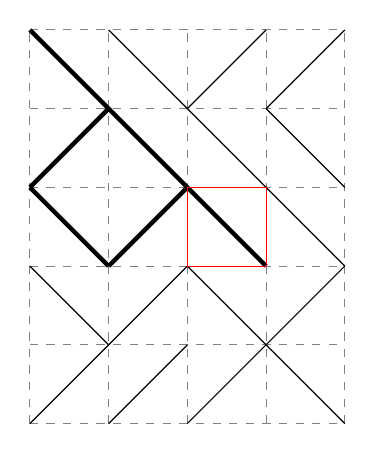
\begin{tikzpicture}
    \draw[thin,gray,dashed] (0,0) grid (4,5);

    \draw[ultra thick] (0,5) -- (1,4);
    \draw[ultra thick] (0,3) -- (1,4); \draw[ultra thick] (1,4) -- (2,3);
    \draw[ultra thick] (0,3) -- (1,2); \draw[ultra thick] (1,2) -- (2,3); \draw[ultra thick] (2,3) -- (3,2);

    \draw (1,5) -- (2,4); \draw (2,4) -- (3,5); \draw (3,4) -- (4,5);
                                                \draw (2,4) -- (3,3); \draw (3,4) -- (4,3);
                                                                      \draw (3,3) -- (4,2);
    \draw (0,2) -- (1,1); \draw (1,1) -- (2,2); \draw (2,2) -- (3,1); \draw (3,1) -- (4,2);
    \draw (0,0) -- (1,1); \draw (1,0) -- (2,1); \draw (2,0) -- (3,1); \draw (3,1) -- (4,0);

    \draw[red] (2,2) -- (2,3);
    \draw[red] (2,3) -- (3,3);
    \draw[red] (3,2) -- (3,3);
    \draw[red] (2,2) -- (3,2);
  \end{tikzpicture}
  \caption{
    An example of a $4 \times 5$ grid, where a segment of size $6$ has been selected.
  }
\end{figure}

\begin{question}
  What is the expected length of the selected segment?
\end{question}

\begin{related}
  \item What is the expected number of segments in an $n \times m$ grid?
  \item How long is the longest segment expected to be?
  \item How does this change if the grid is toroidal, on a cylinder,
    on a M\"obius strip, etc?
\end{related}
\end{document}
